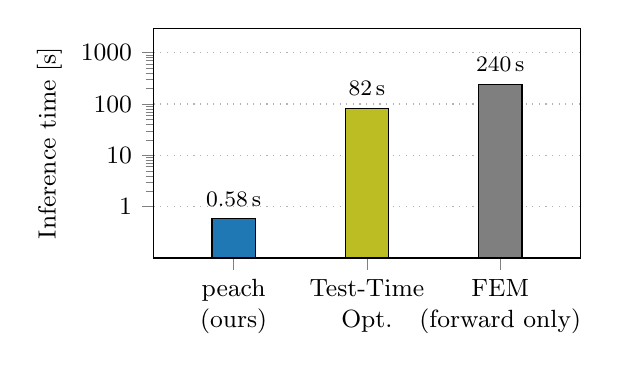
\begin{tikzpicture}
\definecolor{tabblue}{RGB}{31,119,180}
\definecolor{tabolive}{RGB}{188,189,34}
\definecolor{tabgray}{RGB}{127,127,127}

\begin{semilogyaxis}[
  width=7cm,
  height=4.5cm,
  ybar,
  bar width=0.55cm,
  % all bars centered on their own x position (no grouping offset)
  bar shift=0pt,
  % bars start at the lower axis limit instead of at y=1
  log origin=infty,
  ymin=0.1, ymax=3000,
  ytick={1,10,100,1000},
  yticklabels={1,10,100,1000},
  ylabel={Inference time [s]},
  symbolic x coords={PEACH,TTO,FEM},
  xtick={PEACH,TTO,FEM},
  xticklabels={{\gls{peach}\\(ours)}, {Test-Time\\Opt.}, {FEM\\(forward only)}},
  x tick label style={font=\small, align=center},
  enlarge x limits=0.3,
  ymajorgrids,
  grid style={dotted, gray!60},
  tick align=outside,
  ytick pos=left,
  xtick pos=bottom,
  tick label style={font=\small},
  label style={font=\small},
  nodes near coords,
  point meta=explicit symbolic,
  every node near coord/.append style={font=\footnotesize, yshift=1pt},
]
\addplot[fill=tabblue, draw=black, line width=0.5pt]
  coordinates {(PEACH,0.581) [0.58\,s]};
\addplot[fill=tabolive, draw=black, line width=0.5pt]
  coordinates {(TTO,81.93) [82\,s]};
\addplot[fill=tabgray, draw=black, line width=0.5pt]
  coordinates {(FEM,240) [240\,s]};
\end{semilogyaxis}
\end{tikzpicture}